\documentclass[journal,12pt,twocolumn]{IEEEtran}
\usepackage{amsmath,amssymb,amsfonts,amsthm}
\usepackage{txfonts}
\usepackage{tkz-euclide}
\usepackage{listings}
\usepackage{gvv}
\usepackage[latin1]{inputenc}
\usepackage{adjustbox}
\usepackage{array}
\usepackage{tabularx}
\usepackage{enumitem}
\usepackage{pgf}
\usepackage{lmodern}
\usepackage{circuitikz}
\usepackage{tikz}
\usepackage{graphicx}


\begin{document}
\bibliographystyle{IEEEtran}

\vspace{3cm}

\title{}
\author{EE23BTECH11054 -  Sai Krishna Shanigarapu$^{*}$
}
\maketitle
\newpage
\bigskip

\section*{Gate EE 2022}
28. \hspace{2pt}The network shown below has a resonant frequency of 150 kHz and bandwidth of 600
Hz. The Q-factor of the network is \rule{1cm}{0.15mm}\\
(rounded off to one decimal place).\\
\hfill(GATE 2022 EC)\\
\begin{figure}[ht]
  \centering
  \begin{adjustbox}{width=\columnwidth}
      \begin{circuitikz}[american]
    \draw (0,0) to [short, *-] (5,0) to [R=R] (5,2) to [L=L] (5,4) to [short] (2,4) to [C=C] (2,0);
    \draw (0,4) to [short, *-] (2,4);
\end{circuitikz}
  \end{adjustbox}
  \caption{Circuit 1}
\end{figure}\\
\solution\\

\begin{figure}[ht]
  \centering
  \begin{adjustbox}{width=\columnwidth}
      \begin{circuitikz}[american]
    \draw (0,0) to [short, *-] (5,0) to [R=R] (5,2) to [L=$j\omega L$] (5,4) to [short] (2,4) to [C=$\frac{1}{j\omega C}$] (2,0);
    \draw (0,4) to [short, *-] (2,4);
\end{circuitikz}
  \end{adjustbox}
  \caption{Circuit 2}
\end{figure}


\begin{table}[ht]
    \centering
     \begin{adjustbox}{width=\columnwidth}
    \setlength{\arrayrulewidth}{0.3mm}
\setlength{\tabcolsep}{20pt}
\renewcommand{\arraystretch}{1.3}


\begin{tabular}{|c|c|c|}
\hline
Parameter & Description & Value\\
\hline
$f_0$ & Resonant frequency & 150 kHz\\
\hline
$B$ & Bandwidth & 600 Hz\\
\hline
$Q$ & Quality factor & ?\\
\hline
\end{tabular}
    \end{adjustbox}
    \caption{Parameters}
    \label{tab:tab1_gate_ee_2022_28_054}
\end{table}

\begin{table}[ht]
    \centering
     \begin{adjustbox}{width=\columnwidth}
    \setlength{\arrayrulewidth}{0.3mm}
\setlength{\tabcolsep}{20pt}
\renewcommand{\arraystretch}{1.5}


\begin{tabular}{|c|c|c|}
\hline
Parameter & Description & Formula\\
\hline
$Q$ & Quality factor & $\frac{X_L}{R}$\\
\hline
$B$ & Bandwidth & $\frac{R}{2 \pi L}$\\
\hline
$\omega_0$ & Radial resonant frequency & $2 \pi f_0$\\
\hline
$X_L$ & Inductive reactance & $\omega L$\\
\hline
$X_C$ & Capacitive reactance & $\frac{1}{\omega C}$\\
\hline

\end{tabular}

    \end{adjustbox}
    \caption{Formulae}
    \label{tab:tab2_gate_ee_2022_28_054}
\end{table}

At Resonance, 
\begin{align}
    X_L & = X_C\\
    \omega_0 L &= \frac{1}{\omega_0 C}\\
    \omega_0 &= \frac{1}{\sqrt{LC}}\\
    2 \pi f_0 &= \frac{1}{\sqrt{LC}}\\
    \implies f_0 &= \frac{1}{2 \pi \sqrt{LC}} \label{eq:eq1_gate_ee_2022_28_054}    
\end{align}

Using Table \ref{tab:tab2_gate_ee_2022_28_054},
\begin{align}
    Q &= \frac{X_L}{R}\\
    &= \frac{\omega_0 L}{R}\\
    &= \brak{\frac{1}{\sqrt{LC}}}\frac{L}{R}\\
    \implies Q &= \frac{1}{R}\sqrt{\frac{L}{C}} \label{eq:eq2_gate_ee_2022_28_054}
\end{align}

From eq (\ref{eq:eq1_gate_ee_2022_28_054}) and Table \ref{tab:tab2_gate_ee_2022_28_054}
\begin{align}
    \frac{f_0}{B} &= \brak{\frac{1}{2\pi \sqrt{LC}}}\frac{2 \pi L}{R}\\
    &= \brak{\frac{1}{\sqrt{LC}}}\frac{L}{R}\\
    \implies \frac{f_0}{B} &= \frac{1}{R}\sqrt{\frac{L}{C}} \label{eq:eq3_gate_ee_2022_28_054}
\end{align}

From Table \ref{tab:tab1_gate_ee_2022_28_054}, eq (\ref{eq:eq2_gate_ee_2022_28_054}) and eq (\ref{eq:eq3_gate_ee_2022_28_054}),
\begin{align}
    Q &= \frac{f_0}{B}\\
     &=\frac{150 \text{ x } 10^3}{600}\\
    &= 250
\end{align}

$\therefore$ Q-factor is 250

\begin{figure}[ht]
    \centering
    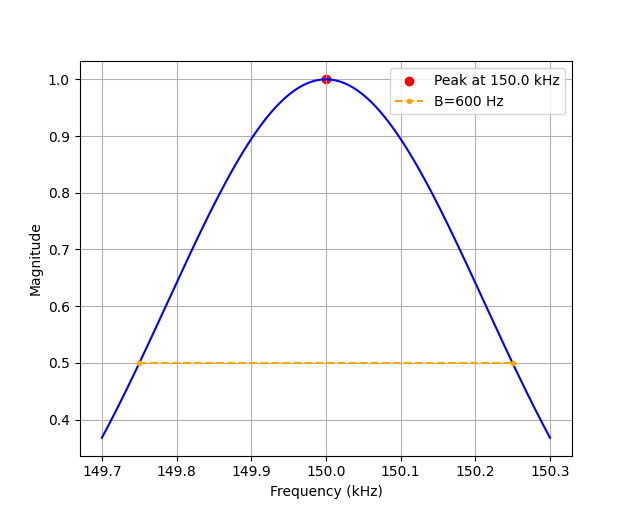
\includegraphics[width=\columnwidth]{figs/Figure_1.png}
    \caption{Plot of Q-factor}
    \label{fig:fig1_gate_ee_2022_18_054}
\end{figure}

\end{document}